\documentclass{article}
\usepackage{amsmath}	%paquete matemática
\usepackage{xtab}		%tablas	
\usepackage{graphicx}	%gráficas
\usepackage{subfigure}	%figuras	
\usepackage{fullpage}	%acomodar página
\usepackage{blindtext}	%texto de relleno
\usepackage{hyperref}	%referencias
\usepackage{multicol}



\author{Guillermo Arag\'on}
\date{\today}
\title{Maxwell's Laws}

\begin{document}
	
	\section{Introducci\'on}
	James Clerk Maxwell\ref{fig:Cara_Maxwell} (Edimburgo, Reino Unido; 13 de junio de 1831-Cambridge, Inglaterra; 5 de noviembre de 1879) fue un físico escocés conocido principalmente por haber desarrollado la teoría electromagnética clásica, sintetizando todas las anteriores observaciones, experimentos y leyes sobre electricidad, magnetismo y aun sobre óptica, en una teoría consistente.1 Las ecuaciones de Maxwell demostraron que la electricidad, el magnetismo y hasta la luz, son manifestaciones del mismo fenómeno: el campo electromagnético. \href{https://es.wikipedia.org/wiki/James_Clerk_Maxwell}{Bibliografía}

	\Blindtext

	\begin{figure}[h!]
		\centering
		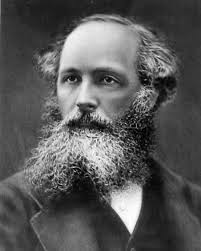
\includegraphics[width=0.35\textwidth]{max1}
		\caption{James Clerk Maxwell}
		\label{fig:Cara_Maxwell}
	\end{figure}

	Las ecuaci\'ones de Maxwell tienen dos formas, la diferencial e integral como se muestra en la \ref{tab:ecuaciones}

	%\begin{equation}
	%\oint\vec{E}\cdot d \vec{A}=\frac{q}{\varepsilon_0}
	%\end{equation}
	
	%\begin{equation}
	%\oint\vec{B}\cdot d \vec{A}=0
	%\end{equation}

	%\begin{equation}
	%\oint\vec{E}\cdot  \vec{ds}=\frac{d\Phi_B}{dt}
	%\end{equation}

	%\begin{equation}
	%\oint\vec{B}\cdot  \vec{ds}=\mu_o i +\frac{1}{c^2} \frac{\partial}{\partial t}\int\vec{E}\cdot d \vec{A}
	%\end{equation}
	

	%\begin{equation}
	%\nabla\cdot{E}=\frac{\rho}{\varepsilon_0}
	%\end{equation}

	%\begin{equation}
	%\nabla\cdot{B}=0
	%\end{equation}

	%\begin{equation}
	%\nabla\times{E}=-\frac{\partial B}{\partial t}
	%\end{equation}

	%\begin{equation}
	%\nabla\times{B}=\frac{J}{\varepsilon_0 c^2}+\frac{1}{c^2}\frac{\partial E}{\partial t}
	%\end{equation}
	\Blindtext

	$\displaystyle\oint\vec{E}\cdot\text{d}\vec{A}=\frac{q}{\varepsilon_0}$&


	\begin{center}
		
	\begin{tabular}{|c|c|}
	\hline \hline
	Integral&Derivada\\
	\hline \hline

	
	$\displaystyle{\oint\vec{E}\cdot\text{d}\vec{A}=\frac{q}{\varepsilon_0}}$&

	
	$\displaystyle{\nabla\cdot{E}=\frac{\rho}{\varepsilon_0}}$
	 \\

	
	$\displaystyle{\oint\vec{B}\cdot d \vec{A}=0}$
	 &

	
	$\displaystyle{\nabla\cdot{B}=0}$
	\\

	\begin{equation*}
	\oint\vec{E}\cdot  \vec{ds}=\frac{d\Phi_B}{dt}
	\end{equation*} &

	\begin{equation*}
	\nabla\times{E}=-\frac{\partial B}{\partial t}
	\end{equation*} \\

	\begin{equation*}
	\oint\vec{B}\cdot  \vec{ds}=\mu_o i +\frac{1}{c^2} \frac{\partial}{\partial t}\int\vec{E}\cdot d \vec{A}
	\end{equation*} &

	\begin{equation*}
	\nabla\times{B}=\frac{J}{\varepsilon_0 c^2}+\frac{1}{c^2}\frac{\partial E}{\partial t}
	\end{equation*} \\

	\hline \hline
	\end{tabular}
	\center	
	\caption{Tabla de Ecuaciones Diferenciales e Integrales}
	\label{tab:ecuaciones}  
	\end{center}

	\begin{multicols}{4}
	\blindtext
	\end{multicols}
\end{document}